\documentclass[11pt]{article}

% Use the following to compile
% mkdir tmp
% pdflatex -aux-directory=tmp -output-directory=tmp --shell-escape notes.tex

% Package use definitions
\usepackage[margin=1in]{geometry} \usepackage{fancyhdr}
\usepackage[parfill]{parskip} \usepackage{graphicx} \usepackage{comment}
\usepackage[outputdir=tmp]{minted} \usepackage[dvipsnames]{xcolor}
\usepackage{listings} \usepackage[hidelinks]{hyperref} \usepackage{amsmath}
\usepackage{amsfonts} \usepackage{amssymb} \usepackage{tcolorbox}
\usepackage{tabu} \usepackage{upgreek} \usepackage[ruled,vlined]{algorithm2e}
\usepackage[nottoc]{tocbibind} \usepackage{natbib}

\setlength{\parindent}{11pt} \setlength{\parskip}{0pt}

% Header and footer setup
\pagestyle{fancy} \rhead{\today} \lhead{Notes}
\renewcommand{\headrulewidth}{1pt} \renewcommand{\footrulewidth}{1pt}

% Image directory specification
\graphicspath{ {./images/} }

% Settings minted option for the entire document
\definecolor{LightGray}{rgb}{0.9, 0.9, 0.9}
\setminted{frame=lines,framesep=2mm,bgcolor=LightGray,linenos,
  fontsize=\footnotesize, baselinestretch=1.2}

% Start of document
\begin{document}

% Title page and table of contents setup
\begin{titlepage}
  \begin{center}
    \vspace*{1cm} \Huge \textbf{ALGOREP Project}\\
    \vspace*{2\baselineskip} \large \textbf{Abstract}
    \vspace*{2\baselineskip}
  \end{center}
  \begin{center}
    \vfill\normalsize \textbf{Gwenegan Bertho}\\ \normalsize \textbf{Kévin
      Guillet}\\ \normalsize \textbf{Mathieu Tammaro}\\ \normalsize \textbf{Jose
      A. Henriquez Roa}\\
    \vspace*{2\baselineskip} \today \rhead{\today}
    \newpage
    \normalsize \tableofcontents
    \newpage
  \end{center}
\end{titlepage}
% Document Body:
\section{Software architecture}
This section shall go though all the design choses made throughout the
development of the project. First, a description of Messenger class, which fully
encapsulates the Open MPI API. Then, an overview of the MessageReceiver virtual
class, followed by a description of the 5 classes inheriting from it, and the
ReceiverManager class that takes care of managing all instanciations of the
derived classes. And finally, a brief description of the Node and Client
classes.
\subsection{Messenger}
\begin{figure}[H]
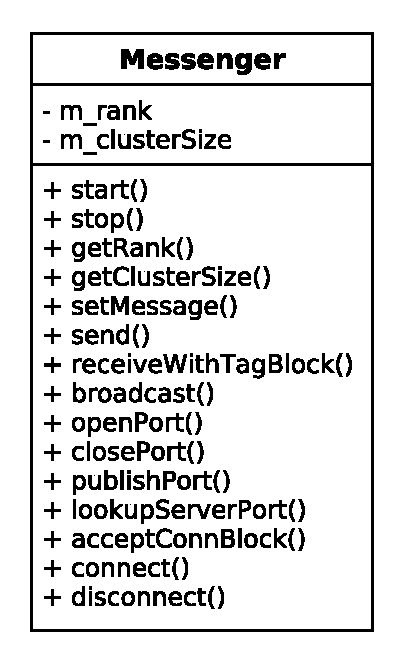
\includegraphics[scale=0.6]{image/messenger.pdf} \centering
\end{figure}
The messenger class, located in \texttt{src/include/messenger.hh}, is a complete
encapsulation of the Open MPI API. All MPI related calls are through the member
functions of this class. When it comes to making use of APIs, the design choice
encapsulating them is fairly common and easily argumented. And as with any
design choice we have done this for the sake of decreasing the complexity of the
overall architecture. Thus, we list some of the benefits of this
encapsulation;\paragraph{}First, it allowed to safely learn to use the API by
localizing any changes made to the program to a single class. Seen as no matter
how much the manual of an API is read, it remains very likely during development
that the use of a given functionality from the API that was previously used
during the early stages might no longer be desired during later stages. For
instance during the development of this project a similar scenario was
encountered were an ambiguity in the MPI standard led to an incorrect assumption
on the behavior of a function; In the 4th version of the Message-Passing
Interface Standard in section \texttt{11.9.3} detailing the client routines to
use when implementing a client/server model with MPI the standard states
that:\\\\ ``\textit{If the port exists, but does not have a pending}
MPI\_COMM\_ACCEPT \textit{, the connection attempt will eventually time out
  after an implementation-defined time, \textbf{or} succeed when the server
  calls} MPI\_COMM\_ACCEPT \textit{.In the case of a time out,}
MPI\_COMM\_CONNECT \textit{raises an error of class } MPI\_ERR\_PORT
\textit{.}''\\\\ This statement differs in the Open MPI documentation, where the
description of the function MPI\_Comm\_Connect states that:\\\\ ``\textit{The}
MPI\_Comm\_connect \textit{call must only be called after the} MPI\_Comm\_accept
\textit{call has been made by the MPI job acting as the server.}''.\\\\ As was
found during the actual use of the MPI\_Comm\_Connect the the highligted 'or' in
the quote from the standard turned out to be an exclusive 'or' where the choice
to either implement the timeout functionality or allow the 'connect' call to
complete upon 'accept' being called on the server was left to the
implementation. This meant that there would be an intrisic need to somehow
handle race conditions from the client, due to the fact that a failed 'connect'
call would eventually timout the client, which would then force the client to
exit with an MPI\_ERR\_PORT error. This was eventually resolved by making the
clients synchronize themselves though the use of an external file, located in
\texttt{etc/turn.txt}. In this scenario this incorrect assumption led to the
unforseen implementation of a client synchonization mechanism. However, if for
instance an incorect assumption had been made on the use of the MPI\_Recv,
causing the need for this call to be switched to the non-blocking variant
MPI\_Irecv. Then having encapsulated the API would then limit the modification
required to be made to a single class, instead of every line thoughout the
project where the function was used.\paragraph{} Another, use for encapsulating
the API is to limit the dependency to said API. For instance, if there ever came
a need to switch Open MPI to another MPI implementation then there would only be
need to switch out the API calls on a single class instead of the entire
project. And the final use for this encapsulation is to simply hide as much
logic related to the API as possible from outside classes. And so be able to
work on other sections of the project without having to keep in mind the usage
of the API and its functionalities. And so, reduce the overall complexity of the
design.
\subsection{MessageReceiver}
\begin{figure}[H]
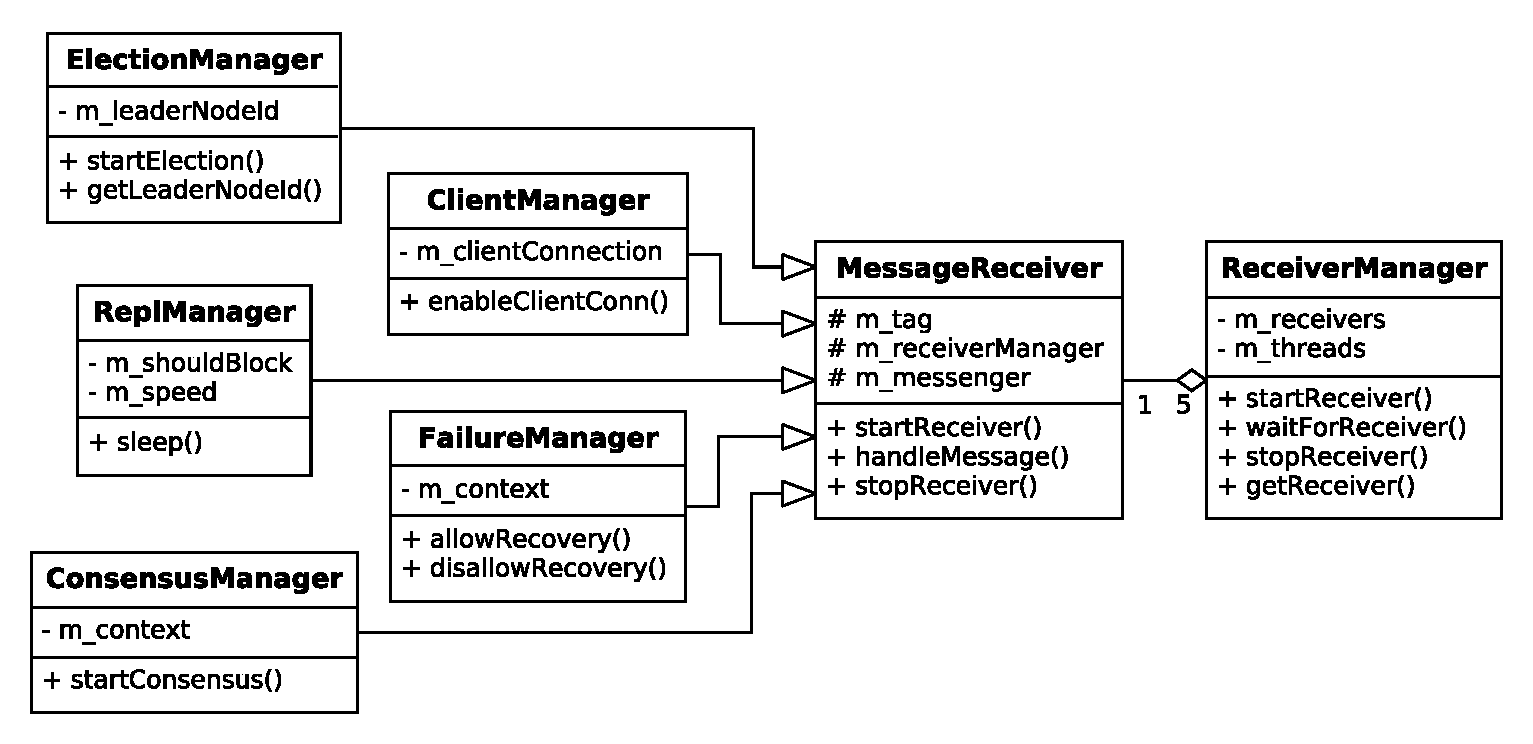
\includegraphics[scale=0.6]{image/receiver.pdf}
\centering
\end{figure}
%% \subsubsection{ConsensusManager}
%% \subsubsection{ElectionManager}
%% \subsubsection{FailureManager}
%% \subsubsection{ClientManager}
%% \subsubsection{ReplManager}
%% \subsection{Node}
%% \begin{figure}[H]
%% 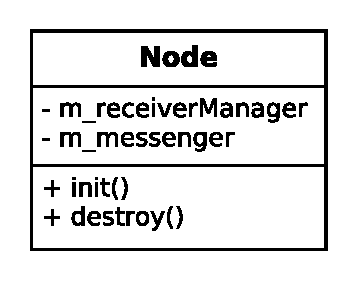
\includegraphics[scale=0.6]{image/node.pdf}
%% \centering
%% \end{figure}
%% \subsection{Client}
%% \begin{figure}[H]
%% 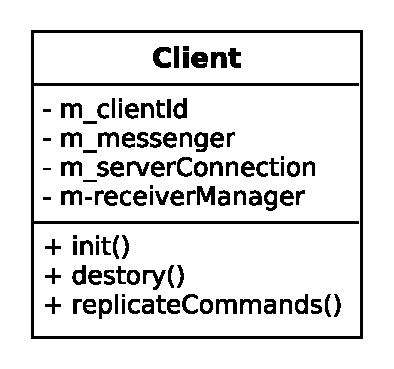
\includegraphics[scale=0.6]{image/client.pdf}
%% \centering
%% \end{figure}
\end{document}
